% !TEX TS-program = pdflatex
% !TEX encoding = UTF-8 Unicode

% This is a simple template for a LaTeX document using the "article" class.
% See "book", "report", "letter" for other types of document.

\documentclass[11pt]{exam} % use larger type; default would be 10pt

\usepackage[utf8]{inputenc} % set input encoding (not needed with XeLaTeX)

%%% Examples of Article customizations
% These packages are optional, depending whether you want the features they provide.
% See the LaTeX Companion or other references for full information.

%%% PAGE DIMENSIONS
\usepackage{geometry} % to change the page dimensions
\geometry{a4paper} % or letterpaper (US) or a5paper or....
\geometry{margin=1in} % for example, change the margins to 2 inches all round
% \geometry{landscape} % set up the page for landscape
%   read geometry.pdf for detailed page layout information

\usepackage{graphicx} % support the \includegraphics command and options

\usepackage[parfill]{parskip} % Activate to begin paragraphs with an empty line rather than an indent

%%% PACKAGES
\usepackage{booktabs} % for much better looking tables
\usepackage{array} % for better arrays (eg matrices) in maths
\usepackage{paralist} % very flexible & customisable lists (eg. enumerate/itemize, etc.)
\usepackage{verbatim} % adds environment for commenting out blocks of text & for better verbatim
\usepackage{subfig} % make it possible to include more than one captioned figure/table in a single float
% These packages are all incorporated in the memoir class to one degree or another...

\usepackage{hyperref}
\usepackage{listings}
\usepackage{xcolor}
\usepackage{color}

\usepackage{xhfill}
\usepackage{amssymb}
\usepackage{textcomp}

\usepackage{minted}
\usepackage[T1]{fontenc}
\usepackage{lmodern}

%%% SECTION TITLE APPEARANCE
\usepackage{sectsty}
\allsectionsfont{\sffamily\mdseries\upshape} % (See the fntguide.pdf for font help)
% (This matches ConTeXt defaults)

%%% ToC (table of contents) APPEARANCE
\usepackage[nottoc,notlof,notlot]{tocbibind} % Put the bibliography in the ToC
\usepackage[titles,subfigure]{tocloft} % Alter the style of the Table of Contents
\renewcommand{\cftsecfont}{\rmfamily\mdseries\upshape}
\renewcommand{\cftsecpagefont}{\rmfamily\mdseries\upshape} % No bold!

%%% END Article customizations

%%% The "real" document content comes below...
\title{Übungen zu EIDI \\ \small \color{blue}Version 1.1.1}
\author{Johannes Stöhr}
%\date{} % Activate to display a given date or no date (if empty),
         % otherwise the current date is printed 


\newcommand{\code}[1]{\mintinline{Java}|#1|}
\newcommand{\fillinline}[1]{\ifprintanswers\fillin[\code{#1}][3cm]\fi\xrfill[-1pt]{0.2mm}}
\newcommand{\fillinlinexl}[1]{\ifprintanswers\fillin[\code{#1}][9cm]\fi\xrfill[-1pt]{0.2mm}}

\renewcommand{\solutiontitle}{\noindent\textbf{Lösung:}\enspace}

\setminted{
    linenos=true,
    frame=single,
    tabsize=4,
}

\usepackage[german]{babel}
\usepackage{csquotes}

\checkboxchar{$\square$}
\checkedchar{$\blacksquare$}

\begin{document}
\maketitle

%\printanswers % ANSWERS

\ifprintanswers
\begin{framed}{\vspace{8.5cm}\begin{center}\color{red}\textbf{ACHTUNG: LÖSUNGEN}\end{center}\vspace{8.75cm}}\end{framed}
\newpage
\fi

\begin{questions}
\question \textbf{Syntaxbäumchen}
\begin{parts}
\part Zeichnen sie ein Syntaxbaum zu folgendem MiniJavaProgramm (mit der Grammatik von PGdP-Blatt 14):\par\nobreak
\begin{minipage}{\linewidth}
\begin{minted}{Java}
int a, b;
int[] c;
b = 42;
a = read();
c = new int[123];
while(a > 0) {
	a = a - 1;
	do {
		c = 12;
	} while(b > length(c));
	if(read() == read()) {
		write(21);
	}
}
\end{minted}
\begin{solution}\par\nobreak
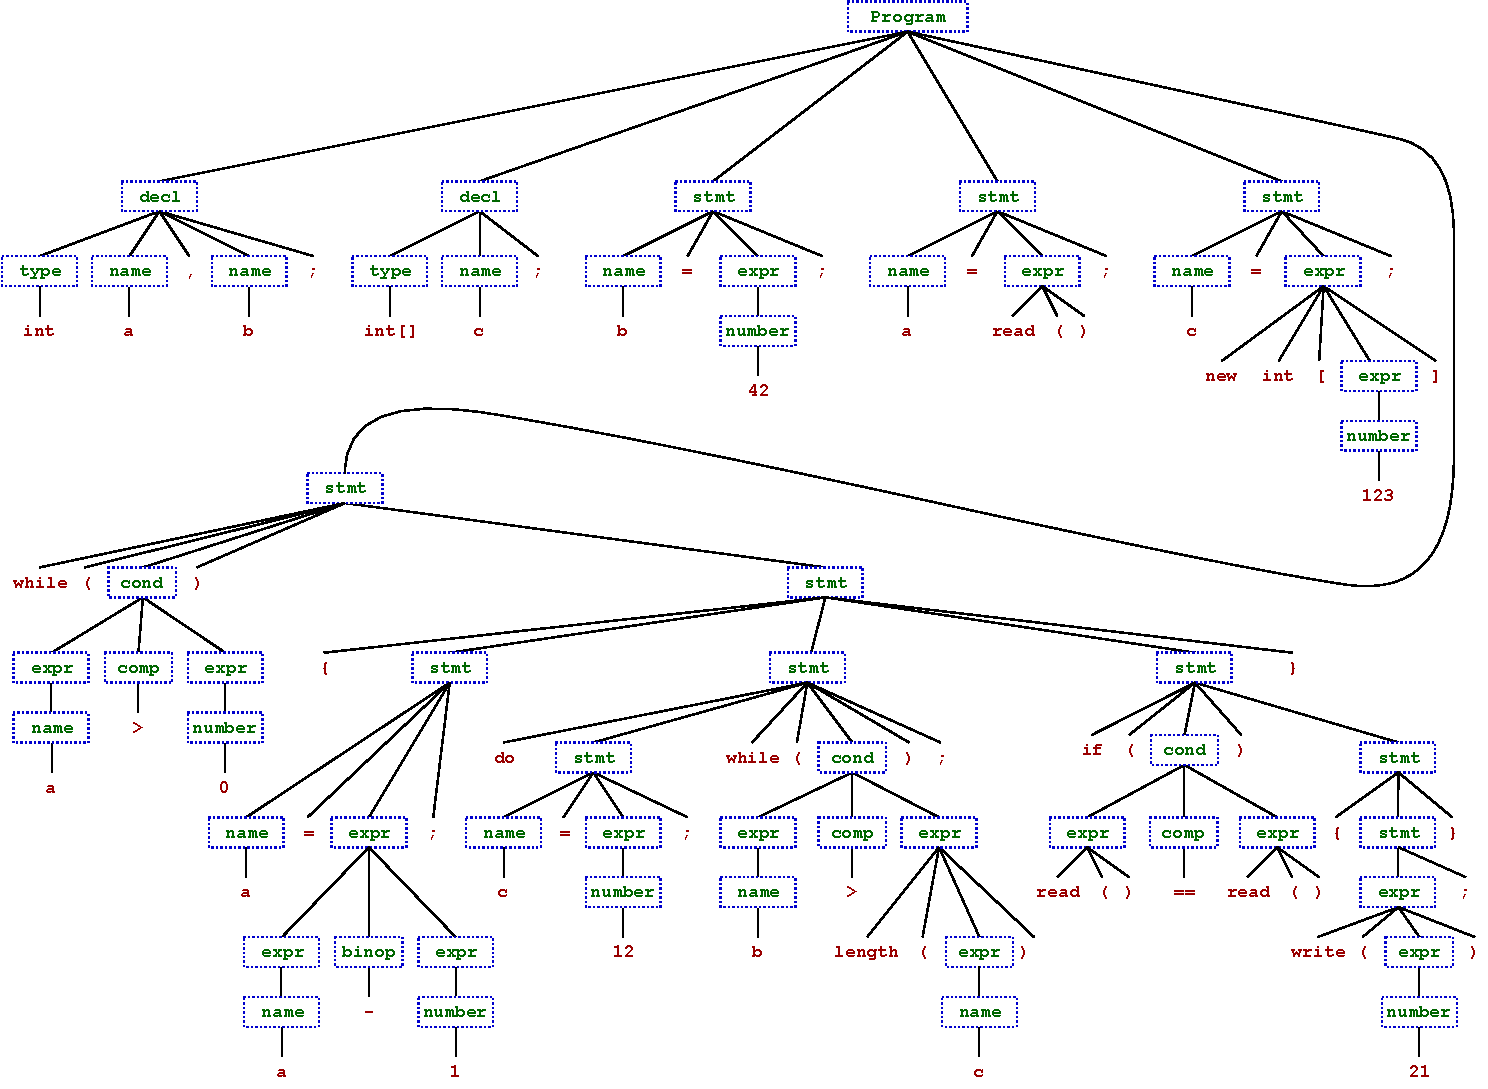
\includegraphics[width=\linewidth]{syntaxbaum.pdf}
\end{solution}
\end{minipage}
\part Würde dieses Programm kompilieren? Warum (nicht)?\par
\nobreak
\begin{solutionordottedlines}[4cm]
Kompiliert, weil es einen gültigen Syntaxbaum gibt und auch der Kontext der Grammatik stimmt, d.h. bei Mini-Java: alle Variablen wurden vorher deklariert. Eine Typprüfung nimmt Mini-Java nicht vor, daher ist das Zuweisen eines \code{int}s zu einem Array wie in Zeile 9 (leider) erlaubt. Die Begründung, dass ein anständiger Compiler so eine Zuweisung nie erlauben dürfte, wäre jedoch auch richtig.
\end{solutionordottedlines}
\end{parts}
\newpage
\question \textbf{Vervollständigen Sie den Lückentext:}\par\nobreak
\begin{minipage}{\linewidth}
\begin{minted}[escapeinside=||]{Java}
public class Randomsort {
	public static void sort(int[] array) {
		while(!isSorted(array)) {
			int index = (|\fillin[int][1cm]|) (Math.random() * (|\fillin[array.length - 1][3.2cm]|)) + |\fillin[1][0.5cm]|;
			// 0.0 <= Math.random() < 1.0
			int remember = |\fillin[array{[index]}][5cm]|;
			array[|\fillin[index][3cm]|] = array[0];
			|\fillin[array{[0]} = remember][7cm]|;
		}
	}
	
	|\fillin[private static boolean][6cm]| isSorted(int[] array) {
		for(|\fillin[int i = 1; i < array.length; i++][8cm]|) {
			if(array[i] < array[i - 1]) {
				return false;
			}
		}
		|\fillin[return true][5cm]|;
	}
}
\end{minted}
\end{minipage}
\question \textbf{Polymorphie}\par\nobreak Was wird bei den folgenden Aufrufen ausgegeben? Betrachten sie jede Ausgabe getrennt von den anderen. Geben Sie an, sofern eine Ausgabe oder Objekterzeugung (\texttt{Obj.Erzeugung}) nicht kompiliert. Sollte eine Exception geworfen werden, soll angegeben werden um welche es sich handelt.
\begin{minted}{Java}
public class Polymorphie {
	public static void main(String[] args) {
		int intOne = 1;
		int intTwo = 3;
		double doubleOne = 3;
		double doubleTwo = 7.0;
		System.out.println(foo(intOne));              // Ausgabe  1
		System.out.println(foo(doubleTwo));           // Ausgabe  2
		System.out.println(foo(intTwo, intOne));      // Ausgabe  3
		System.out.println(foo(doubleOne, intTwo));   // Ausgabe  4
		System.out.println(foo(intOne, doubleOne));   // Ausgabe  5
		A a = new A();                                // Obj.Erzeugung 1
		B b1 = new B();                               // Obj.Erzeugung 2
		B b2 = new B(b1);                             // Obj.Erzeugung 3
		C c1 = new C();                               // Obj.Erzeugung 4
		C c2 = new C(b2);                             // Obj.Erzeugung 5
		// Sehr viele; nicht unbedingt alle für die Übung,
		// manche auch für Zuhause, wenn man nochmal üben will
		System.out.println(a.goo(a));                 // Ausgabe  6
		System.out.println(a.goo(b2));                // Ausgabe  7
		System.out.println(a.goo(c2));                // Ausgabe  8
		System.out.println(a.goo(new E()));           // Ausgabe  9
		System.out.println(b1.goo(b1));               // Ausgabe 10
		System.out.println(b2.goo(a));                // Ausgabe 11
		System.out.println(b1.equals(b2.goo(b2)));    // Ausgabe 12
		System.out.println(c2.goo(a, b2));            // Ausgabe 13
		System.out.println(c2.goo(b1, a));            // Ausgabe 14
		System.out.println(c2.hoo());                 // Ausgabe 15
		b1 = new C(b2);                               // Obj.Erzeugung 6
		System.out.println(b1.goo(b1));               // Ausgabe 16
		System.out.println(b1.goo(b2));               // Ausgabe 17
	}

	private static double foo(double a, double b) {
		return a > b ? a : b;
	}

	private static int foo(double a, int b) {
		return foo((int) a);
	}

	private static int foo(int a, double b) {
		return (int) foo((double) a, b);
	}

	private static int foo(int a) {
		return 4 * a + 2;
	}

	public static class A {
		public String toString() {
			return "A";
		}

		public A goo(A a) {
			return new A();
		}

		public C goo(D d) {
			return (C) d;
		}
	}

	public static class B extends A {
		public B b;

		public B(B b) {
			this.b = b;
		}

		public B() {
			b = null;
		}

		public String toString() {
			return "B";
		}

		public A goo(B b) {
			return this.b;
		}

		public B goo(A a, B b) {
			return (B) b.goo(a);
		}
	}

	public static class C extends B implements D {
		public C(B b) {
			super(b);
		}

		public String toString() {
			return "C";
		}

		public A goo(A a) {
			return a.goo(a);
		}

		public A goo(B b) {
			return new B(null);
		}

		public A goo(B b, A a) {
			return a.goo(b);
		}

		public B hoo() {
			return new B(this.b);
		}
	}

	public interface D {
		public B hoo();
	}

	public static class E implements D {
		public B hoo() {
			return new C(null);
		}
	}
}
\end{minted}
\begin{solution}
Text in der Konsole oder Fehlergründe je Ausgabe:\par\nobreak
\begin{enumerate}
\item \code{6}\par
\item Kompiliert nicht, es gibt keine Methode \code{Polymorphie.foo(double)} oder eine kompatible Überladung.\par
\item Kompiliert nicht, beide Methoden \code{Polymorphie.foo(int, double)} und \newline\code{Polymorphie.foo(double, int)} kommen in Frage und keine ist näher an \newline\code{foo(int, int)} als die jeweils andere. (mehrdeutiger Methodenaufruf)\par
\item \code{14}\par
\item \code{3}\par
\item \code{A}\par
\item \code{A}\par
\item Kompiliert nicht, da \code{A.goo(A)} und \code{A.goo(D)} beide ein \code{C}-Objekt entgegennehmen können, weil \code{C} Subtyp von \code{A} ist und \code{D} implementiert. Wie bei 3. ein mehrdeutiger Methodenaufruf.\par
\item Wirft zur Laufzeit eine \code{ClassCastException}, weil \code{E} zwar auch \code{D} implementiert, aber keine Unterklasse von \code{C} ist. Das neu erzeugte \code{E}-Objekt kann somit nicht zu \code{C} gecastet werden.
\item \code{null}\par
\item \code{A}\par
\item \code{true}\par
\item Es wird eine \code{ClassCastException} geworfen, weil das in \code{A.goo(A)} erzeugte \code{A}-Objekt in der Methode \code{B.goo(A, B)} zu \code{B} gecastet werden kann. \code{B} ist Unterklasse von \code{A} , aber nicht umgekehrt.
\item \code{A}\par
\item \code{B}\par
\item \code{B}\par
\item \code{B}\par
\end{enumerate}
Zudem kompiliert Objekterzeugung 4 nicht, weil es keinen parameterlosen Konstruktor in der Klasse \code{C} gibt.
\end{solution}
\question \textbf{Pingus Space Odyssey}\par\nobreak
Pingu ist im Weltall unterwegs. Allerdings wurde sein Raumschiff von einem Weltraumeisbären angegriffen, weshalb er nun zum Flottenstützpunkt muss, um sich auf einen Gegenschlag vorzubereiten.\par
Dafür muss er sich durch den Weltraum bewegen, in dem es mehrere Beacons gibt. Jeder dieser
Punkte ist mit einem oder mehreren anderen Punkten verbunden. Dies wird durch eine
Adjazenzmatrix dargestellt. Das ist ein zweidimensionales int-Feld, in dem jeweils eine Verbindung
von einem Punkt (Zeilenindex) zu einem anderen Punkt (Spaltenindex) an der jeweiligen Stelle
durch eine „1“ gekennzeichnet ist. Es sind auch Schleifen und „Einbahnstraßen“ möglich!
Jedoch gibt es auch Wurmlöcher als Verbindung, die mit einer „2“ gekennzeichnet sind. Diese
erzeugen eine Kopie von Pingu (neuer Thread) in einem Paralleluniversum an dem Zielpunkt des
Wurmlochs, der normale Pingu bleibt an seinem Punkt und kann sich frei einen anderen Weg
aussuchen.\par
Jedoch müssen die Grenzen der Paralleluniversen gewahrt werden, daher dürfen zwei Kopien von
Pingu nicht am selben Beacon existieren, da sonst die beiden Realitäten kollidieren und alles
auseinandergerissen wird.\par
Damit Pingu nicht im Kreis fliegt, sollte sich jede Kopie von ihm merken, wo diese schonmal war.
Wird Pingu kopiert weiß die neue Kopie nichts vom bisherigen Weg. Nur für die Bonusaufgabe darf der bisherige Weg übergeben werden.
Sollte Pingu in einer Sackgasse landen, darf er einen Schritt zurückgehen und von dort einen
anderen Weg wählen. Sollten alle Wege von einem Punkt nicht zum Ziel führen, darf er noch einen
Schritt weiter zurückgehen und so weiter.\par
Sobald eine Kopie von Pingu das Ziel erreicht hat, können alle Pingus aufhören nach einem Weg
zu suchen, da die Sternenflotte ein spezielles Funkgerät besitzt, mit dem sie auch mit
Paralleluniversen kommunizieren kann. Daher sind dann automatisch alle Pingukopien gerettet.\par
Erweitern sie hierzu die Implementierung der Klasse \code{PenguinAstronaut}.\par
\emph{Bonus: Ein Erzähler schildert nach Pingus Ankunft die aufregende Reise durch das Weltall.}\par
\begin{minipage}{\linewidth}
\begin{minted}{Java}
public class Space {
	// 0 = keine Verbindung; 1 = Verbindung; 2 = Wurmloch
	private int[][] adjacencyMatrix; 

	public int[][] getAdjacencyMatrix() {
		return adjacencyMatrix;
	}
	
	public Space(int[][] adjacencyMatrix) {
		this.adjacencyMatrix = adjacencyMatrix;
	}
	
	public static void main(String[] args) {
		//Nur ein Beispiel
		int[][] matrix = { { 0, 0, 2 }, { 0, 0, 0 }, { 0, 1, 1 } };
		Space space = new Space(matrix);
		PenguinAstronaut pingu = new PenguinAstronaut(space, 0, 2);
		pingu.start();
	}
}

public class PenguinAstronaut extends Thread {
	public PenguinAstronaut(Space s, int from, int to) {
		// "Standardkonstruktor" für main() in Space
	}
}
\end{minted}
\end{minipage}
\ifprintanswers
\filbreak
\textbf{Mögliche Lösung:}\par\nobreak
\begin{minted}[breaklines,breakindent=20pt]{Java}
import java.util.ArrayList;
import java.util.List;

public class PenguinAstronaut extends Thread {
	private static Object[] locks;

	private static synchronized void initLocks(int size) {
		// Initialise lock objects only once
		if (locks == null) {
			locks = new Object[size];
			for (int i = 0; i < locks.length; i++) {
				locks[i] = new Object();
			}
		}
	}

	private Space space;
	private int sizeOfSpace;
	private int start;
	private int to;
	private boolean[] visited;

	// For stopping all Threads at the end
	private PenguinAstronaut parentThread;
	private List<PenguinAstronaut> childThreads;

	// For telling the way afterward
	private List<Integer> visitedLocations;

	// Standard constructor for first Pingu
	public PenguinAstronaut(Space space, int start, int to) {
		this(space, start, to, null, new ArrayList<>());
	}

	// Constructor for every other Pingu
	public PenguinAstronaut(Space space, int start, int to, PenguinAstronaut parentThread, List<Integer> visitedLocs) {
		this.space = space;
		sizeOfSpace = space.getAdjacencyMatrix().length;
		this.start = start;
		this.to = to;
		visited = new boolean[sizeOfSpace];

		this.parentThread = parentThread;
		childThreads = new ArrayList<>();

		this.visitedLocations = visitedLocs;

		initLocks(sizeOfSpace);
	}

	@Override
	public void run() {
		visit(start);
	}

	private void visit(int index) {
		// Way was already found
		if (this.isInterrupted())
			return;

		// Needs to be declared before synchronized
		int nextVisit = 0;
		// Lock current location
		synchronized (locks[index]) {
			// Found location of starfleet
			if (index == to) {
				tellStory();
				stopSearching(this);
				return;
			}
			visitedLocations.add(index);
			visited[index] = true;

			/*
			 * New Pingus through wormholes 
			 * 
			 * matrix[index][i] = 1 means there is a way from
			 * the current location to the beacon with the index i
			 */
			for (int i = 0; i < sizeOfSpace; i++) {
				if (space.getAdjacencyMatrix()[index][i] == 2 && !visited[i]) {
					PenguinAstronaut p = new PenguinAstronaut(space, i, to, this, new ArrayList<>(visitedLocations));
					childThreads.add(p);
					p.start();
				}
			}
			// Visit next beacons
			nextVisit = nextVisit(nextVisit, index);
		}

		while (nextVisit != -1) {
			visit(nextVisit);
			// We're back from a dead end
			synchronized (locks[index]) {
				visitedLocations.remove(visitedLocations.size() - 1);
				// Determine if and where to go next
				nextVisit = nextVisit(nextVisit + 1, index);
				// Possibly going back one step, unlock current beacon
			}
		}
	}

	private int nextVisit(int seachStart, int index) {
		// Looking for the next Place to visit
		for (int i = seachStart; i < sizeOfSpace; i++) {
			if (space.getAdjacencyMatrix()[index][i] == 1 && !visited[i])
				return i;
		}
		return -1;
	}

	private void stopSearching(PenguinAstronaut stopping) {
		// Stop parent if it's not the one stopping
		if (parentThread != null && parentThread != stopping) {
			parentThread.stopSearching(this);
		}
		// Stop every child that is not the one stopping
		for (PenguinAstronaut p : childThreads) {
			if (p != stopping) {
				p.stopSearching(this);
			}
		}
		// Interrupt this Pingu's search
		this.interrupt();
	}

	private void tellStory() {
		for (Integer i : visitedLocations) {
			System.out.println("I was at beacon " + i);
		}
	}
}
\end{minted}
\fi
\end{questions}
\end{document}